\definecolor{fig-color-i}{RGB}{ 191, 236, 255}
\definecolor{fig-color2}{RGB}{  144, 221, 255}
\definecolor{fig-color3}{RGB}{  103, 209, 255}
\definecolor{fig-color4}{RGB}{   49, 192, 255}
\definecolor{fig-color-ri}{RGB}{  0, 177, 255}
\begin{center}
  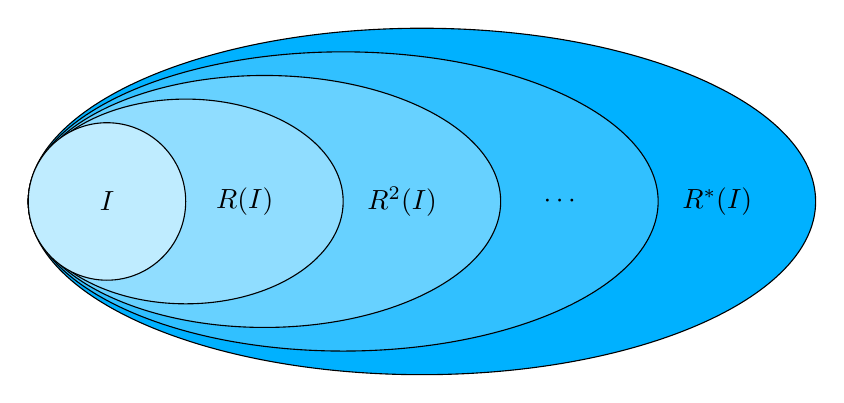
\begin{tikzpicture}
    \draw[fill=fig-color-ri] (4,0) ellipse (5 and 2.2);
    \node (r*i) at (7.75,0) {$R^*(I)$};
    
    \draw[fill=fig-color4] (3,0) ellipse (4 and 1.9);
    \node (...) at (5.75,0) {$\cdots$};
    
    \draw[fill=fig-color3] (2,0) ellipse (3 and 1.6);
    \node (r2i) at (3.75,0) {$R^2(I)$};
    
    \draw[fill=fig-color2] (1,0) ellipse (2 and 1.3);
    \node (ri) at (1.75,0) {$R(I)$};
    
    \draw[fill=fig-color-i] (0,0) ellipse (1 and 1);
    \node (i) at (0,0) {$I$};
  \end{tikzpicture}
\end{center}
  